\documentclass{beamer}

\usepackage{graphicx}
\usepackage{amsmath}
\usepackage{amsfonts}
\usepackage{amssymb}
\usepackage{listings}
\usepackage{tikz}
\definecolor{mygray}{rgb}{0.92,0.92,0.92}
\usetheme{Montpellier}
\usecolortheme{beaver}


\begin{document}


\section{Group Meeting}
\title{Group Meeting \\ Week 2, Spring 2019}
\author{Brandon Gusto} %
\institute{Dept. of Scientific Computing \\ Florida State University}
\date{\today}
\frame{\titlepage}

\section{Finite Volume}

\begin{frame}[center]{Finite Volume Approach}
    Here we consider the following one-dimensional reference PDE
    \begin{equation*}
      w_{t} + f(w)_{x} = s(w)
    \end{equation*}
    where $w = (\rho,\rho u,E)$ represents the primitive solution variables, and initial and boundary
    conditions are supplied. The PDE in semi-discrete form (via finite volume w/ midpoint quadrature) is
    \begin{equation*}
          (w_{j})_{t} = -\frac{1}{h} \left( f_{j+\frac{1}{2}} - f_{j-\frac{1}{2}} \right) + s_{j}
                      = R_{j}(w)
    \end{equation*}
    where the $j$ denotes spatial index.
\end{frame}

\begin{frame}[center]{Finite Volume Approach}
    The numerical flux at cell interface is a function of $2k$ local cells
    \begin{equation*}
          \hat{f}_{j+\frac{1}{2}} = f(w^{n}_{j-k+1},\dots,w^{n}_{j+k})
    \end{equation*}
    The solution is represented as cell averages
    \begin{equation*}
          w^{n}_{j} \approx \frac{1}{\triangle x} \int_{x_{j-\frac{1}{2}}}^{x_{j+\frac{1}{2}}} w(x,t_{n}) dx
    \end{equation*}
\end{frame}

\section{Multiresolution}

\begin{frame}[center]{Multiresolution Representation}
    Define multiple, nested grids
    \begin{equation*}
      G^{l} = \left\{ x^{l}_{j} \right\}_{j=0}^{N_{l}}
    \end{equation*}
    such that $x_{j}^{l} = x_{2j}^{l-1}$ for any $j,l$. The number of cells per level $l$ is $N_{l}$
    and the cell width is
    \begin{equation*}
      h_{l} = \frac{b-a}{N_{l}}
    \end{equation*}
\end{frame}


\begin{frame}[center]{Multiresolution Representation}
	Consider some quantity $c(x)$ represented as cell averages $c_{j}^{l}$ at each
	level $l$. At some level $l$ (coarse) the field at level $l-1$ (fine) is represented by a prediction from
	values at level $l$.
	\begin{figure}
    \centering
    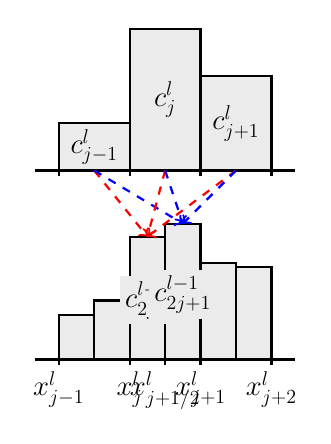
\begin{tikzpicture}[thick,scale=0.3, every node/.style={scale=0.6}]
		\draw[fill=mygray] (0,0) -- (0,2)-- (3,2) -- (3,0);
		\draw[fill=mygray] (3,0) -- (3,6) -- (6,6) -- (6,0);
		\draw[fill=mygray] (6,0) -- (6,4) -- (9,4) -- (9,0);
		\draw[fill=mygray] (-1,0) -- (10,0);
		\node at (1.5,1) {\LARGE $c^{l}_{j-1}$};
		\node at (4.5,3) {\LARGE $c^{l}_{j}$};
		\node at (7.5,2) {\LARGE $c^{l}_{j+1}$};
		\draw (0,0) -- (0,-0.25);
		\draw (3,0) -- (3,-0.25);
		\draw (6,0) -- (6,-0.25);
		\draw (9,0) -- (9,-0.25);

		% -8 is y-axis baseline for this one
		\draw[fill=mygray] (0,-8) -- (0,-6.1) -- (1.5,-6.1) -- (1.5,-8);
		\draw[fill=mygray] (1.5,-8) -- (1.5,-5.5) -- (3,-5.5) -- (3,-8);
		\draw[fill=mygray] (3,-8) -- (3,-2.8) -- (4.5,-2.8) -- (4.5,-8);
		\draw[fill=mygray] (4.5,-8) -- (4.5,-2.25) -- (6,-2.25) -- (6,-8);
		\draw[fill=mygray] (6,-8) -- (6,-3.9) -- (7.5,-3.9) -- (7.5,-8);
		\draw[fill=mygray] (7.5,-8) -- (7.5,-4.1) -- (9,-4.1) -- (9,-8);
		\draw[fill=mygray] (-1,-8) -- (10,-8);
		\node[fill=mygray] at (3.75,-5.5) {\LARGE $c^{l-1}_{2j}$};
		\node[fill=mygray] at (5.25,-5.25) {\LARGE $c^{l-1}_{2j+1}$};
		\draw (0,-8) -- (0,-8.25);
		\draw (3,-8) -- (3,-8.25);
		\draw (4.5,-8) -- (4.5,-8.25);
		\draw (6,-8) -- (6,-8.25);
		\draw (9,-8) -- (9,-8.25);

		% arrows
		\draw[red,dashed,->] (1.5,0) -- (3.75,-2.8);
		\draw[blue,dashed,->] (1.5,0) -- (5.25,-2.25);
		\draw[red,dashed,->] (4.5,0) -- (3.75,-2.8);
		\draw[blue,dashed,->] (4.5,0) -- (5.25,-2.25);
		\draw[red,dashed,->] (7.5,0) -- (3.75,-2.8);
		\draw[blue,dashed,->] (7.5,0) -- (5.25,-2.25);

		% ticj text
		\node[below] at (0,-8.25) {\LARGE $x^{l}_{j-1}$};
		\node[below] at (3,-8.25) {\LARGE $x^{l}_{j}$};
		\node[below] at (4.5,-8.25) {\LARGE $x^{l}_{j+1/2}$};
		\node[below] at (6,-8.25) {\LARGE $x^{l}_{j+1}$};
		\node[below] at (9,-8.25) {\LARGE $x^{l}_{j+2}$};

	    \end{tikzpicture}
	\end{figure}

\end{frame}


\begin{frame}[center]{Multiresolution Representation}
    Using a standard third-order polynomial, the prediction in one-dimension is
    \begin{align*}
      \hat{c}^{l-1}_{2j} = c^{l}_{j} + \frac{1}{8} \left( c^{l}_{j-1} - c^{l}_{j+1} \right) \\
      \hat{c}^{l-1}_{2j+1} = c^{l}_{j} - \frac{1}{8} \left( c^{l}_{j-1} - c^{l}_{j+1} \right)
    \end{align*}
    and the detail coefficient for the cell corresponding to $c^{l}_{j}$ is
    \begin{equation*}
      d^{l}_{j} = c_{2j+1}^{l-1} - \hat{c}_{2j+1}^{l-1}
    \end{equation*}
    The value of this coefficient is indicitive of the smoothness of the function in that
    vicinity.
\end{frame}


\section{Multiresolution Code}

\begin{frame}[center]{Multiresolution Code - Examples}
	\begin{figure}
		\center
		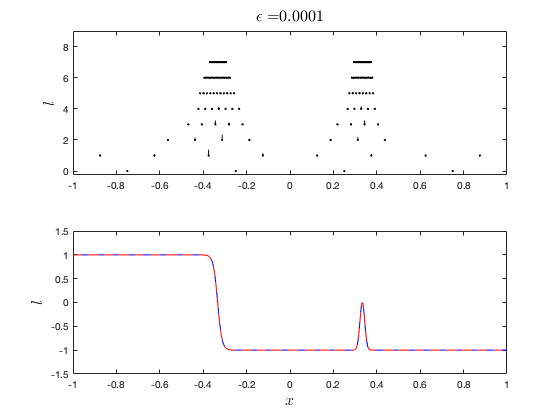
\includegraphics[scale=0.5]{plots/spike-med.png}
		\caption{Better approximation (smaller threshold value).}
	\end{figure}
\end{frame}

\section{Multiresolution Finite Volume Scheme}

\begin{frame}[center]{Multiresolution Scheme on AMR Patches}
	\begin{figure}
		\center
		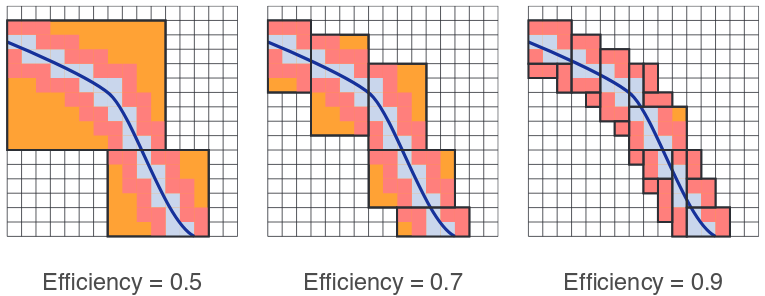
\includegraphics[scale=0.5]{plots/patch-efficiency.png}
		\caption{Increasing patch 'efficiency.'}
	\end{figure}
\end{frame}

\begin{frame}[center]{Multiresolution Scheme on AMR Patches}
      The steps of the scheme for one patch are
      \begin{enumerate}
        \item take given (finest level) data on patch, and coarsen it to desired coarsest level $L$
        \item compute the forward wavelet transform to obtain $\left\{ \mathbf{d}^{l}\right\}_{l=L}^{l=1}$
        \item on coarsest level $L$, compute the residuals $\left\{ R_{j}^{L} \right\}_{j=0}^{N_{L}}$
        \item loop through one finer level at a time, and according to detail coefficients,
              either interpolate or calculate remaining fluxes
      \end{enumerate}
\end{frame}

\begin{frame}[center]{Multiresolution Scheme on AMR Patches}
  The original (fine) data is coarsened by
      \begin{equation*}
        w_{j}^{l} = \frac{1}{2} \left( w_{2j}^{l-1} + w_{2j+1}^{l-1} \right)
      \end{equation*}
      Then the residual $R_{j}^{l}$ may be interpolated in smooth regions as
      \begin{align*}
        R^{l-1}_{2j+1} & = R^{l}_{j} - \frac{1}{8} \left( R^{l}_{j-1} - R^{l}_{j+1} \right) \\
        R^{l-1}_{2j} & = 2 R^{l}_{j} - R^{l-1}_{2j+1}
      \end{align*}
\end{frame}

\begin{frame}[fragile,center]{Progress in FLASH Implementation}
  \begin{itemize}
    \setlength\itemsep{1em}
    \item created a new folder \texttt{source/flashUtilities/Wavelet/}
    \item writing a program \texttt{Wavelet\_computeTransform.F90} which will be run 
          in \texttt{Grid\_computeUserVars.F90}
  \end{itemize}
  \begin{verbatim}
    function imap( l, i, j, k, nx, ny, nz ) result(x)
      integer, intent(in) :: nx(:), ny(:), nz(:)
      integer, intent(in) :: l, i, j, k
      integer             :: x

      ! compute the map
      x = l + nx * ( i + ny * ( j + nz * k ) )

    end function imap
  \end{verbatim}
\end{frame}


\end{document}
